\documentclass[11pt]{article}

\newcommand{\cnum}{CM146}
\newcommand{\ced}{Fall 2018}
\newcommand{\ctitle}[3]{\title{\vspace{-0.5in}\cnum, \ced\\Problem Set #1: #2}}
\usepackage{enumitem}
\newcommand{\solution}[1]{{{\color{blue}{\bf Solution:} {#1}}}}
\usepackage[usenames,dvipsnames,svgnames,table,hyperref]{xcolor}
\usepackage{graphicx}
\graphicspath{ {./images/} }
\usepackage{amsmath}
\usepackage{subfig}
\usepackage{siunitx}
\usepackage{amssymb}

\renewcommand*{\theenumi}{\alph{enumi}}
\renewcommand*\labelenumi{(\theenumi)}
\renewcommand*{\theenumii}{\roman{enumii}}
\renewcommand*\labelenumii{\theenumii.}


\begin{document}
\title{CM146, Fall 2018 \\ Problem Set 2: Perceptron and Regression}
\author{Gajan Nagaraj}
\date{10	/11/2018}
\maketitle
\vspace{-0.75in}

\section*{Problem 4}
Visualization:

\begin{enumerate}[label=(\alph*)]
\item We adjust $plot\_data(...)$ in order to visualize the training and test data. 
\centerline{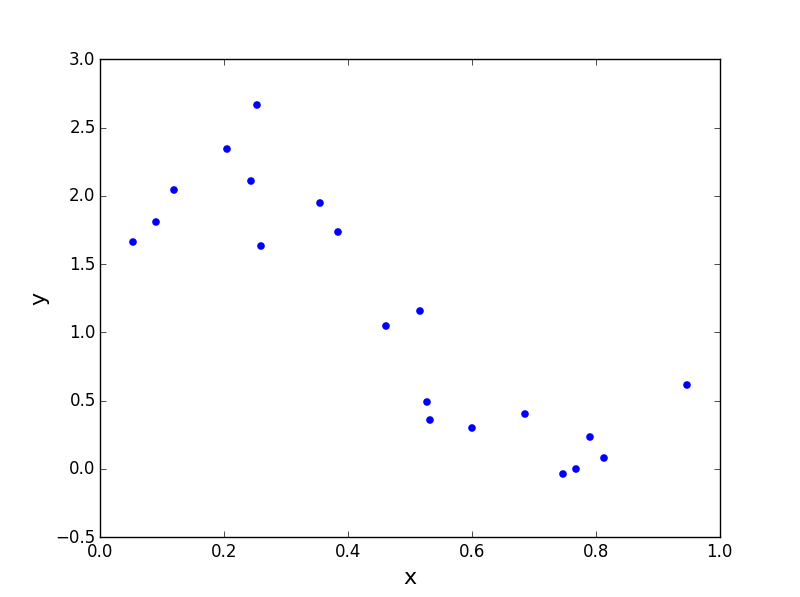
\includegraphics[scale=.7]{part_a_train}} 
\centerline{Fig 1: Training data visualized using $plot\_data(...)$}
\centerline{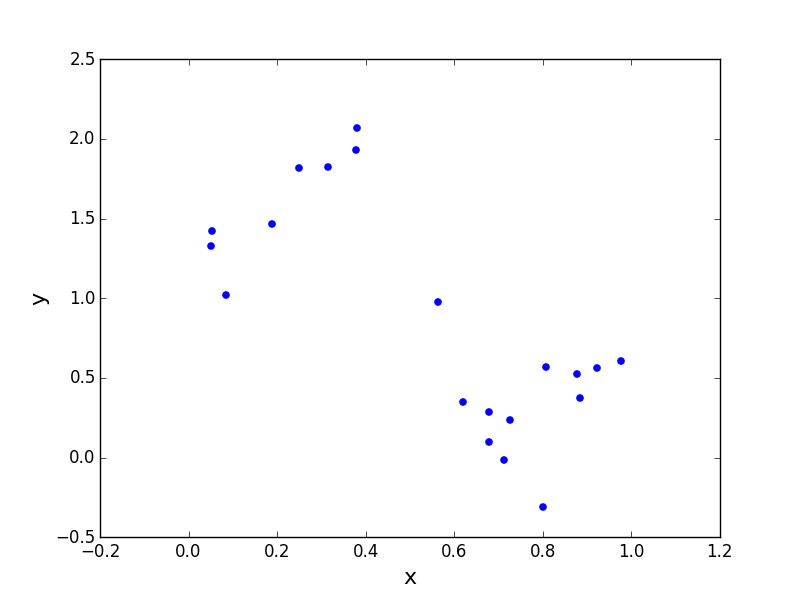
\includegraphics[scale=.7]{part_a_test}} 
\centerline{Fig 2: Test data visualized using $plot\_data(...)$}
I noticed that the training data (Fig 1) has a linear correlation, thus a function can be found to fit the data. However, I also noticed that linear regression will be ineffective for the test data (Fig 2) because there is extremely weak linear correlation in the test data. This means that we could draw a line to fit the training data (and predict values for based of it). If we attempted to do the same with the test data, then our predictions would have a large margin of error.
\end{enumerate}
Linear Regression:
\begin{enumerate}[resume]
\item I modified $PolynomialRegression.generate\_polynomial\_features(...)$ to create the matrix
$X$ for a simple linear model in the code and got the expected output.
\item I completed $PolynomialRegression.predict(...)$ in the code to predict $y$ from $X$ and $w$.
\item I completed $PolynomialRegression.cost(...)$ to calculate $J(w)$ and got the expected output (40.234).
Next, I implemented the gradient descent step in $PolynomialRegression.fit\_GD(...)$ per the spec. I then tested different $\eta$ and made a table of the coefficients, number of iterations until convergence and the final value of the objective function.
\begin{center}
    \begin{tabular}{| l | l | l | l | l |}
    \hline
    $\eta$ & Iterations & Cost & Coefficients & Time \\ \hline
    $10^{-4}$ & 10000 & 4.086 & [2.270 -2.461] & 0.413\\ \hline
    $10^{-3}$ & 7021 & 3.913 & [2.446 -2.816] & 0.328\\ \hline
    $10^{-2}$ & 765 & 3.913 & [2.446 -2.816] & 0.032\\ \hline
    $0.0407$ & 10000 & \num{2.711e+39} & [\num{-9.405e+18} \num{-4.652e+18}] & 0.419\\ \hline
    \end{tabular}
\end{center}
From the table we can see that the coefficients for $10^{-4}$ and $0.0407$ did not converge to the actual weights. We can see that as the step got around  $10^{-3}$ and $10^{-2}$, the coefficients converged to [ 2.27044798 -2.46064834]. We see that for $0.0407$, the coefficients and cost are very weird numbers. This makes sense because the step size is too big, thus the gradient descent calculation is unstable and does not provide with an accurate solution. We see that a step size of $10^{-4}$ and $0.0407$ took $10000$ iterations to converge while $10^{-3}$ took $7021$ iterations, and $10^{-2}$ only took $765$ iterations to converge. This means that $10^{-2}$ converges the fastest.

\item I implemented the closed-form solution $PolynomialRegression.fit(...)$ in the code. The closed form solution is the computer calculated from my code is [2.446 -2.816]. The cost of the closed form solution calculation is 3.913. We can see that the coefficients and cost are identical to GD using $\eta = 10^{-3}$ and $\eta = 10^{-2}$. The algorithm runs much faster than GD. When we run the code, we can see that because there are no iterations done, the code executes instantly. After timing the closed form solution, we can see that it completed in $0.001$ seconds. This is much faster compared to all off the GD calculations seen above.

\item I then set a learning rate $\eta$ for GD that is a function of the number of iterations. Specifically, I set it to $\eta_{k} = \frac{1}{1+k}$. \\I updated $PolynomialRegression.fit\_GD(...)$ with the new learning rate. The new algorithm takes $10000$ iterations to converge. The algorithm obtained coefficients of [2.270 -2.461] and cost of 4.086. We can see that this is the same as before with a specified $\eta = 10^{-4}$. I also timed this function and it took $0.417$ seconds to run. 
\end{enumerate} 
Polynomial Regression:
\begin{enumerate}[resume]
\item I updated $PolynomialRegression.generate\_polynomial\_features(...)$ in the code to create an $m + 1$ dimensional feature vector for each instance.

\item I implemented $PolynomialRegression.rms\_error(...)$ to calculate the Root Mean Square Error. We use RMSE when calculating error because it allows us to measure error on the same scale with the same units as $y$. Additionally, we can use RMSE as a measure of the spread of the y values around the regression line. If RMSE is zero, then we can expect all our data points lie exactly on our regression line. If it is not, then that means there is some deviation of the data points from the regression line.

\item I modified the code so that it would determine the best-fit solver polynomial regression solver on the training and test data. The code generated the following graph which depicts how RSME varies with the model complexity: \\
\centerline{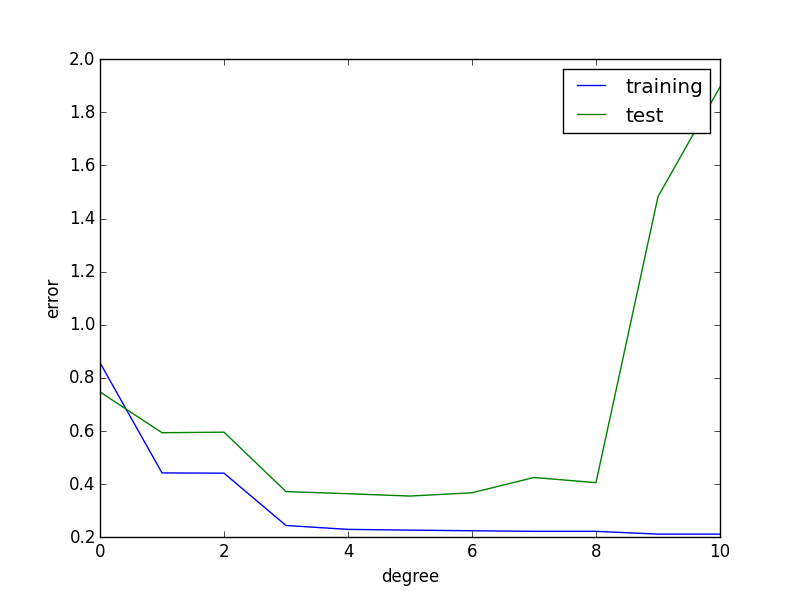
\includegraphics[scale=.7]{part_i_plot}} 
\centerline{Fig 3: RSME vs. Model Complexity}
According to Fig 3, I would say that degree 5 polynomial best fits the data because that is where the test RMSE was the lowest at a value of $0.35$. We notice that as the degree increases, the training RMSE decreases while the test RMSE increases. Thus, we must observe where the test RMSE is the lowest to determine what degree is the best. There is evidence of overfitting the data in the graph. Around degree 8, we can see that the training and test RMSE diverge (with training RMSE decreasing and test RMSE increasing). From this, we can conclude that as the degree of the polynomial increases, the polynimial model overfits to the training data and thus we get a sudden large test RMSE error.

\end{enumerate}
\end{document}
